% Requires \usepackage{graphicx}. Put the PDF next to the main .tex file.
\begin{figure*}[p]
  \centering
  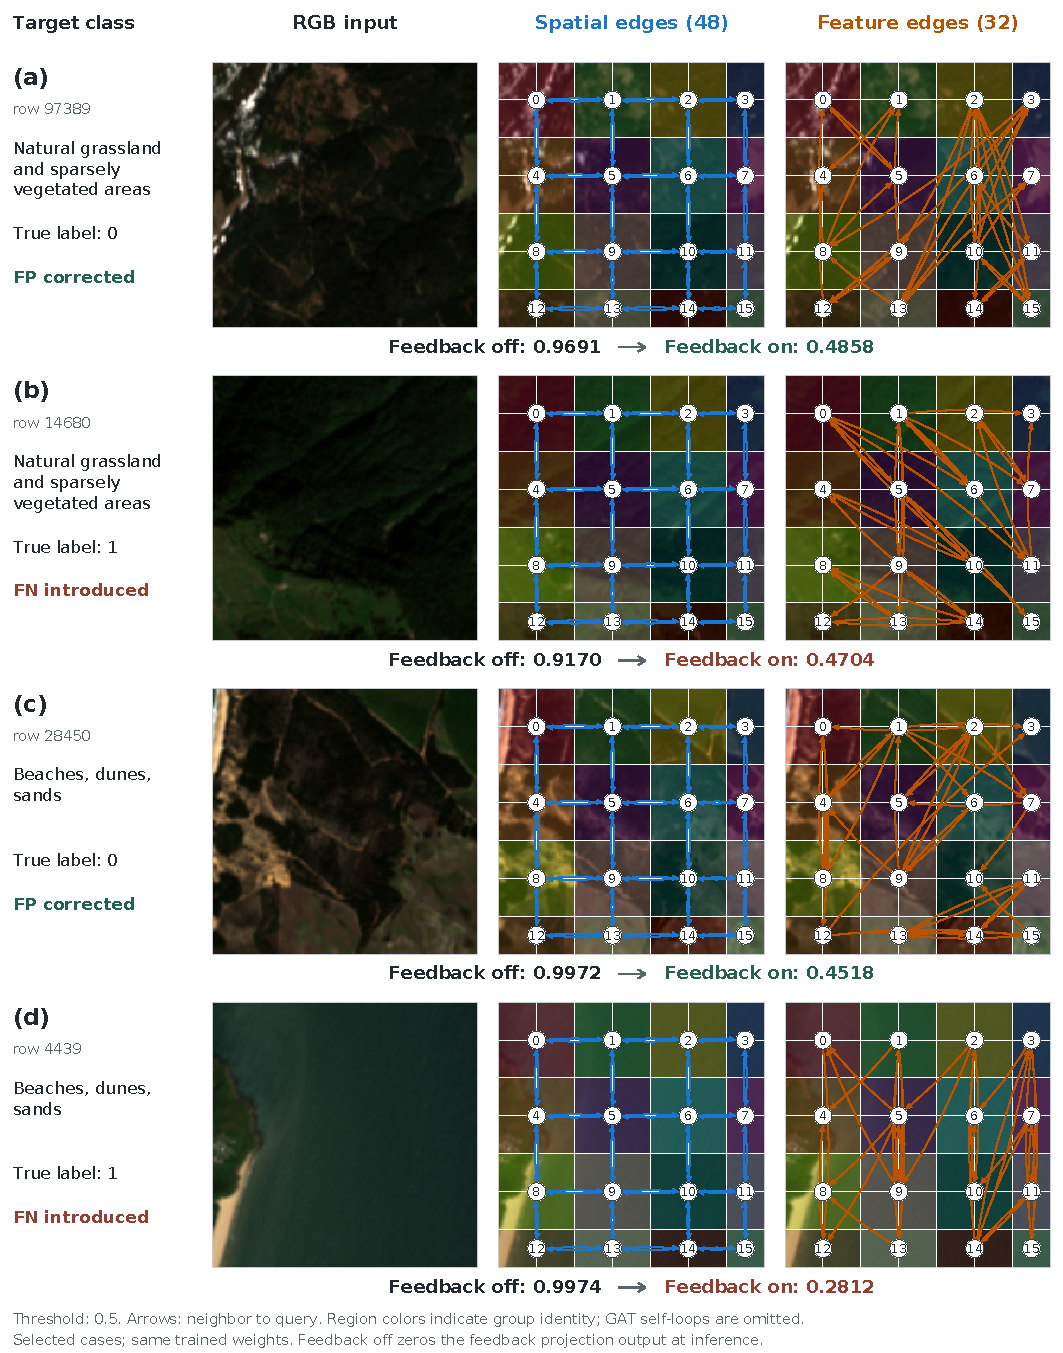
\includegraphics[width=\textwidth,height=0.82\textheight,keepaspectratio]{gavit_seed44_feedback_cases.pdf}
  \caption{Graph-feedback interventions on fixed BigEarthNet-19 validation cases using GAViT trained with seed 44. Each row shows the RGB input, region assignments with spatial edges, and region assignments with feature edges. Directed edges were captured from the normal forward pass and point from a neighboring region to the query region. Blue and orange denote 48 spatial and 32 additional feature edges; internal GAT self-loops are omitted. Target-class probabilities use the same trained weights, with feedback retained or the output of the feedback projection set to zero, at a threshold of 0.5. Retained feedback corrects false positives in (a,c) but introduces false negatives in (b,d). These cases comprise all four threshold flips among 24 previously fixed diagnostic images. Selected cases do not estimate population performance; zero-feedback inference is not a retrained graph-free baseline, and the edges do not establish edge-specific causal attribution.}
  \label{fig:gavit-feedback-cases}
\end{figure*}
